\chapter{Development of the algorithm for NP research}
\label{chap:Z_5D}





In this Chapter the foundations of the algorithm employed for data analysis will be carefully explained step by step. A good practice is to begin from the statistical foundation of the algorithm itself as it is set on not trivial concepts. In the next step, a network shall be built for the purpose beginning from its architecture and then choosing proper activation functions, optimizer and weight initialization. Moreover, several crucial aspects that may cause difficulties in the work progression will be highlighted and faced in order to find the best solution or at least a compromise, if there isn't. Some of the problems that shall be faced are:
\begin{itemize}
	\item The search for the number of degrees of freedom of the network employed.
	\item The look-elsewhere effect.
	\item The limitation of the phase-space of the NN free parameters, which means clipping the weights.
\end{itemize}





\section{Statistical foundations}
The entire construction of the statistical foundations of the procedure is accurately described in \cite{wulzer} for a monodimensional case. Here we recap the main steps to the construction of a hypotesis test and so of a variable with discriminating power, but for a multidimensional case. However, the logical passages remain unchanged.



\subsection{Construction of a test statistic}
The starting point is a dataset of repeated measurements of a $d$-dimensional random variable $x$, distributed as the reference distribution $n(x|\R)$. To compare the reference distribution with observed data an alternative hypostesis is needed, which means another distribution $n(x|\mathbf{w})$. It is convenient to parametrize $n(x|\mathbf{w})$ in terms of $n(x|\R)$. Moreover, we know that $n(x|\mathbf{w})$ is strictly positive and since the log-likelihood ratio will be used later, we will express it as:
\begin{equation}
	n(x|\mathbf{w}) = n(x|\R) e^{f(x;\mathbf{w})}
\end{equation}
where $f(x)$ is a function from a set $\mathcal{F} = \{ f(x;\mathbf{w}), \forall \mathbf{w} \}$.

Now that the set of alternative hypoteses is built in a parametrized form, the optimal statistical test for the reference model is defined by the Neyman-Pearson construction, which is based on the maximum likelihood principle\footnotemark. The idea is to compare $n(x|\R)$ with the best fit distribution $n(x|\hat{\mathbf{w}})$, where $\hat{\mathbf{w}}$ is the one that maximizes the likelihood. Hence the test statistic is:
\begin{equation}
	\label{eqn:T}
	t(\mathcal{D})
	=
	2 \log{\left[
	\frac{\mathcal{L}_{\hat{\mathbf{w}}}}{\mathcal{L}_{\R}}
	\right]}
	= 
	2 \log{\left[
	\frac{e^{-N(\hat{\mathbf{w}})}}{e^{-N(\R)}} \prod_{x \in \mathcal{D}} \frac{n(x|\hat{\mathbf{w}})}{n(x|\R)}
	\right]}
	=
	-2 \min_{\{\mathbf{w}\}}{\left[
	N(\mathbf{w}) - N(\R) - \sum_{x \in \mathcal{D}} f(x;\mathbf{w})
	\right]}
\end{equation}
where $N(\R)$ is the expected number of events in the reference model and $N(\mathbf{w})$ is the expected number of events in the alternative hypotesis. $N(\mathbf{w})$ can be computed by:
\begin{equation}
	N(\mathbf{w}) = \int n(x|\mathbf{w}) \d x = \int n(x|\R) e^{f(x;\mathbf{w})} \d x
\end{equation}
The test statistic needs a consistent definition of a $p$-value. In order to compute it, we have to associate a probability to the value of $t$, denominated as $t_\mathrm{obs}$, obtained using the observed dataset. For this reason we also have to find the PDF of $t$ in the reference hypotesis and we can do it by evaluating $t$ a sufficient number of times on a large sample of toy datasets. By this way, we can obtain the observed $p$-value:
\begin{equation}
	p_\mathrm{obs} = \int_{t_\mathrm{obs}}^{\infty} P(t|\R) \d t
\end{equation}

The key idea of \cite{wulzer}, employed for the present work, is to parametrize the alternative hypotesis with neural networks for their properties of universal unbiased approximants.

\footnotetext{
Let's suppose we are performing a hypotesis test between two simple hypotesis $H_{0} = \{\theta = \theta_{0}\}$ and $H_{1} = \{\theta = \theta_{1}\}$ using the likelihood-ratio test:
\begin{equation}
	\Lambda(x) := \frac{\mathcal{L}(\theta_{0}|x)}{\mathcal{L}(\theta_{1}|x)}
\end{equation}
with a threshold $\eta$, for which $H_{0}$ is rejected in favour of $H_{1}$ at a significance level of $\alpha = P(\Lambda(x) \le | H_{0})$. Then, the Neyman-Pearson lemma states that $\Lambda(x)$ is the most powerful test at significance level $\alpha$.
}

\subsection{Ideal test statistic}
The results of the method that exploits the power of neural networks must be discussed in comparison with something we already know. It means that assuming we have complete knowledge of the distribution describing the observed data, an ideal test statistic could be defined and it will be the previous cited benchmark.

The alternate hypotesis with the assumption of complete knowledge will be denoted by 'NP' and it has no free parameters. In this case the test statistic becomes:
\begin{equation}
	t_\mathrm{id}(\mathcal{D})
	=
	2 \log{\left[
	\frac{\mathcal{L}_{\NP}}{\mathcal{L}_{\R}}
	\right]}
	=	
	2 \log{ 
	\left[
	\frac{e^{-N(\NP)}}{e^{-N(\R)}}
	\prod_{x \in \mathcal{D}} \frac{n(x|\NP)}{n(x|\R)}
	\right]
	}
\end{equation}
According to the Neyman-Pearson lemma, $t_\mathrm{id}$ is the optimal discriminant between the reference and the new physics hypotheses. It produces the smallest median $p$-value if NP is the true distribution of the data sample. From this value, the ideal significance can be computed as stated in \cite{cowan}:
\begin{equation}
	\sigma_\mathrm{id}
	=
	\sqrt{t_\mathrm{id}}
	=	
	\sqrt{
	2 \log{\left[
	\frac{\mathcal{L}_{\NP}}{\mathcal{L}_{\R}}
	\right]}
	}
\end{equation}

This test statistic is denoted as 'ideal' because it is the most suited one to discover data departures from the reference model. However, it is not useful but as a benchmark because we can use it only when the true data distribution is known a priori. In our case we are testing the efficiency of a ML-approach and therefore the true distribution is known.



\subsection{Adaptation of $t(\mathcal{D})$ as a loss function}
The minimization in Equation \ref{eqn:T} must be done numerically through the tools for neural network training discussed in Chapter \ref{chap:NN}. Before doing this, we have to express Equation \ref{eqn:T} as a loss function.

The first thing to do is to estimate $N(\mathbf{w})$. This task can be done through Monte Carlo methods:
\begin{equation}
	N(\mathbf{w}) = \frac{N(\R)}{N_{\mathcal{R}}} \sum_{x \in \mathcal{R}} e^{f(x;\mathbf{w})}
\end{equation}
Thus Equation \ref{eqn:T} becomes:
\begin{equation}
	t(\mathcal{D}) = -2 \min_{\{\mathbf{w}\}}{\left[
	\frac{N(\R)}{N_{\mathcal{R}}} \sum_{x \in \mathcal{R}} (e^{f(x;\mathbf{w})} -1) -
	\sum_{x \in \mathcal{D}} f(x;\mathbf{w})
	\right]}
	\equiv
	-2 \min_{\{\mathbf{w}\}}{\left[ f(\cdot,\mathbf{w}) \right]}
\end{equation}
$L$ has the form of a loss function. It is convenient to write it as a single sum over events by introducing a target variable $y$ such that:
\begin{itemize}
	\item $x \in \mathcal{R} \Longrightarrow y=0$;
	\item $x \in \mathcal{D} \Longrightarrow y=1$.
\end{itemize}
Thus the explicit expression of $L$ is:
\begin{equation}
	L[f] = \sum_{(x,y)} \left[
	(1-y) \frac{N(\R)}{N_{\mathcal{R}}} (e^{f(x)} - 1) - yf(x)
	\right]	\label{eqn:LOSS}
\end{equation}

The trained neural network, denoted with its output $f(x;\hat{\mathbf{w}})$, is simply the maximum likelihood fit to the data and reference distributions log-ratio. It is the best approximant of the true underlying data distribution $n(x|\T)$:
\begin{equation}
	f(x;\hat{\mathbf{w}}) \approx \log{ \left[
	\frac{n(x|\T)}{n(x|\R)}
	\right] }
\end{equation}


\section{The algorithm}
The network architecture chosen for the task has the following characteristics:
\begin{itemize}
	\item 3 fully-connected layers, with the first and the second ones with five neurons each and the last one with only one output neuron. Therefore the input is multidimensional since the input is the set of HLFs (except for the invariant mass $M_{Z}$) for every event.
	\item The activation functions chosen are sigmoids for the first and second layer, while a linear activation is employed for the last layer.
\end{itemize}

The loss function employed is reported in the previous section in Equation \ref{eqn:LOSS} and it is a cross entropy loss function adapted for the task. Its minization is done by \textsc{AdaM} algorithm. The initialization of the free parameters is the normal random initialization. A clip to the weights is applied in the case they go out of a prearranged interval. The discussion on the weight clipping is studied in deeper in the subsequent sections.

The scheme of the algorithm is the following:
\begin{itemize}
	\item A sufficiently large reference sample is randomly selected from the whole dataset following the reference distribution. Then a data sample with background events is randomly selected from the entire dataset and no signal is added. The network is trained with these data and the output of the process is the minimized loss function. From this value, the final $t$ is computed as minus two times the minimized loss function.
	\item The previous step is repeated a certain number of times in order to sample the distribution of $t$ in the reference hypotesis (as no signal event is added in the data sample yet). The desidered number of $t$ necessary to the following steps must be considered carefully because the procedure is computationally expensive and its complexity grows linearly with the number of events in the reference sample.
	\item When the distribution of $t$ in the reference hypotesis is sampled, the first step is repeated but adding a certain number of signal events in the data sample. The output of the process, i.e. the minimized loss, is translated into the value of $t_\mathrm{obs}$.
	\item The distribution of $t$ and $t_\mathrm{obs}$ are used to compute a $p$-value $p$, which is the area under the tail.
	\item If the value of $p$ is sufficiently small, it signals a tension with the reference hypotesis. Hence anomalies are detected and they can be analyzed through the log-ratio $f(x;\hat{\mathbf{w}})$.
\end{itemize}





\section{Computing resources}
Suppose one wants to sample 200 values of $t$ in the reference hypotesis. Moreover, suppose that the execution of a single process to obtain a single value of $t$ takes about 1 day. It is clear that doing this task on a single machine is computationally very expensive. Assuming this machine could run 10 processes at the same time without swapping, it would take 20 days to get the desired results. Considering the entire procedure has to be repeated for different conditions and for several numbers of events in the reference sample, it is totally inconceivable to do everything on a single machine.

Another aspect has to been taken into account. Writing the code that executes the algorithms described above could be quite tricky and unavoidable mistakes in the phase of implementation don't agree with the long execution time if we want to check the results for every change.

In this section a solution for each of these difficulties encountered is presented.



\subsection{\textsc{TensorFlow} back-end and \textsc{Keras} API}
The programming language chosen for the work is \textsc{Python 3}. Its simplicity and power were crucial in the selection. Moreover, there exists very powerful tools that address machine learning problems and which can make the code easier to write and understand.

The API employed for the task is \textsc{Keras}, which is an open source library specialized for automatic learning tasks. It was used with \textsc{TensorFlow} as back-end. The ladder is the most common machine learning library up to now and it provides tools not only for deep learning problems, but for every machine learning problem conceivable. For more information, see \cite{python}, \cite{keras} and \cite{tensorflow}.

A bunch of code to build the network and to train it is reported below to give an idea of its clarity. In the following example the architecture of the net is (5,5,1) and the code is reported in a simplificated version.

\begin{lstlisting}[frame=single]
import keras

inputs= keras.layers.Input(shape=(5,))
dense = keras.layers.Dense(5, activation='sigmoid')(inputs)
dense = keras.layers.Dense(5, activation='sigmoid')(dense)
output= keras.layers.Dense(1, activation='linear')(dense)

model = Model(inputs=[inputs], outputs=[output])

model.compile(loss=Loss,
              optimizer='adam')

model.fit(x_train, 
          y_train,
          epochs=300000,
          batch_size=batch_size,
          verbose=0,
          shuffle=False)
\end{lstlisting}



\subsection{LSF and clustering}
In order to speed up the sampling of $t$ distribution, the algorithm was parallelized on a cluster of machines. This is to be intended that different processes were executed simultaneously on different machines and not that a single process was executed on more machines.

The machines used for the task are sited in Legnaro and Padua. The processes sent to them are called \texttt{bjobs} and the sending procedure is done by LSF, which stands for Load Sharing Facilities. Every bjob must be sent by a script, launched through \texttt{bsub} command. Before doing this, a configuration procedure of the machine, through which the jobs were dispatched, has to be done. To make this procedure easier, the access to this machine was done through cloudveneto. A virtual machine instance was created and connected to the lsf sender. It was then personalized to run a python script with these functionalities:
\begin{itemize}
	\item It configures the environment variables of the machines in order to let the necessary packages accessible by the system. This phase was accomplished by the execution of another script accessible on cvmfs (CERN Virtual Machine File System). More informations on this tool are provided in \cite{cvmfs}.
	\item It creates the script that sends the job via LSF to the machines. This phase is executed a number of times equal to the number of toy samples, therefore equal to the number of $t$ values we want.
\end{itemize}

The jobs sent to the machines are placed with their IDs in a queue. For this work, cms-local-queues were used, listed in Table \ref{tab:QUEUES}.

\begin{table}[H]
	\centering
	\begin{tabular}{c c c}
		\toprule
		Queue name	&	Max job number	&	Max job runtime	\\
		\midrule
		local-cms-short	&	500			&	1440 min		\\
		local-cms-long	&	300			&	10080 min		\\
		\bottomrule
	\end{tabular}
	\caption{Available queues.}
	\label{tab:QUEUES}
\end{table}

\noindent
Since the complexity scales up linearly with the number of events in the reference sample, runtime for jobs with wide reference sample overtake the limit of 1440 minutes of the short queue. Therefore the long queue was a better choice for the task. A list of the machines accessible by this queue and their characteristics are displayed in Table \ref{tab:LONG_QUEUE_MACHINES}.

\begin{table}[H]
	\centering
	\begin{tabular}{c c c c}
	\toprule
	Machine id	&	Number of CPUs	&	Max Memory		&	Max Swap	\\
	\midrule
	\texttt{wp-05-01}	&	2	&	64554M  &	8191M	\\
	\texttt{wl-07-01}	&	2	&	64537M  &	8191M	\\
	\texttt{wl-07-02}	&	2	&	64537M  &	8191M	\\
	\texttt{wl-07-03}	&	2	&	64537M  &	8191M	\\
	\texttt{wl-07-04}	&	2	&	64537M  &	8191M	\\
	\texttt{wl-07-05}	&	2	&	64537M  &	8191M	\\
	\texttt{wl-07-06}	&	2	&	64537M  &	8191M	\\
	\texttt{wl-07-07}	&	2	&	64537M  &	8191M	\\
	\texttt{wl-07-08}	&	2	&	64537M  &	8191M	\\
	\texttt{wl-07-09}	&	2	&	64537M  &	8191M	\\
	\texttt{wl-07-10}	&	2	&	64537M  &	8191M	\\
	\bottomrule
	\end{tabular}
	\caption{Machines and resources.}
	\label{tab:LONG_QUEUE_MACHINES}
\end{table}





\section{Degrees of freedom of the network}
Trying to understand the exact number of the degrees of freedom of a neural network is not a trivial task. This number must reflect the wideness of the space of functions the network can span. A more complex network will obviously be characterized by a larger number of dof.

A possible approach to determine the number of dof starts from the free parameters of the network. If there are $n$ weight parameters and $m$ biases, the number of dof $\nu$ can be estimated by:
\begin{equation}
	\nu = n + m
\end{equation}

Therefore, given the network architecture, the number of layers, neurons and the activations, we can give a definition adapted to the case we are studying. A scheme of the network employed is given in Figure \ref{fig:DOF}, which makes easier to understand how the connections between different layers work and the way data flow through the net.

\begin{figure}[H]
    \centering
    % DOF of Neural Network
\begin{tikzpicture}[shorten >=1pt,->,draw=black!50, node distance=\layersep, scale=0.8]
    \tikzstyle{every pin edge}=[<-,shorten <=1pt]
    \tikzstyle{neuron}=[circle,fill=black!25,minimum size=15pt,inner sep=0pt]
    \tikzstyle{input neuron}=[neuron, fill=green!50];
    \tikzstyle{sigmoid}=[neuron, fill=cyan!50]
    \tikzstyle{output neuron}=[neuron, fill=red!50];
    \tikzstyle{hidden neuron}=[neuron, fill=blue!50];
    \tikzstyle{annot} = [text width=5em, text centered]

    % Draw the input layer nodes
    \foreach \name / \y in {1,...,5}
    % This is the same as writing \foreach \name / \y in {1/1,2/2,3/3,4/4}
        \node[input neuron, draw=black!100, thick, pin=left:{\scriptsize In{[}\#\y{]}}] (I-\name) at (-3.0*\layersep,\y) {};

    % Draw the input layer nodes
    \foreach \name / \y in {1,...,5}
    % This is the same as writing \foreach \name / \y in {1/1,2/2,3/3,4/4}
        \node[sigmoid, draw=black!100, thick] (S1-\name) at (-1.0*\layersep,\y) {$\sigma$};

    % Draw the hidden layer nodes
    \foreach \name / \y in {1,...,5}
        \node[hidden neuron, draw=black!100, thick] (H-\name) at (\layersep,\y) {};

    % Draw the input layer nodes
    \foreach \name / \y in {1,...,5}
    % This is the same as writing \foreach \name / \y in {1/1,2/2,3/3,4/4}
        \node[sigmoid, draw=black!100, thick] (S2-\name) at (3.0*\layersep,\y) {$\sigma$};

    % Draw the output layer node
    \node[output neuron, draw=black!100, thick, pin={[pin edge={->}]right:{\scriptsize Out{[}\#1{]}}}, right of=S2-3] (O1) {$\propto$};

    % Connect every node in the input layer with every node in the
    % hidden layer.
    \foreach \source in {1,...,5}
        \foreach \dest in {1,...,5}
            \path (I-\source) edge (S1-\dest);

    % Connect every node in the input layer with every node in the
    % hidden layer.
    \foreach \source in {1,...,5}
    	\foreach \dest in {1,...,5}
        	\path (S1-\source) edge (H-\dest);

    % Connect every node in the input layer with every node in the
    % hidden layer.
    \foreach \source in {1,...,5}
        \foreach \dest in {1,...,5}
            \path (H-\source) edge (S2-\dest);

    % Connect every node in the input layer with every node in the
    % hidden layer.
    \foreach \source in {1,...,5}
        \path (S2-\source) edge (O1);

    % Annotate the layers
    \node[annot,above of=I-5, node distance=1.0cm] (ail) {Input layer};
    \node[annot,above of=S1-5, node distance=1.0cm] (as1) {Sigmoid};
    \node[annot,above of=H-5, node distance=1.0cm] (ahl) {Hidden layer};
    \node[annot,above of=S2-5, node distance=1.0cm] (as2) {Sigmoid};
    \node[annot,right of=as2] {Output layer};
    
    \node[annot,below of=S1-1, node distance=1.0cm] (bs1) {\textbf{25} weights\\\textbf{5} biases};
    \node[annot,below of=H-1, node distance=1.0cm] (bhl) {\textbf{25} weights\\\textbf{5} biases};
    \node[annot,below of=S2-1, node distance=1.0cm] (bs2) {\textbf{25} weights\\\textbf{5} biases};
    \node[annot,right of=bs2] {\textbf{5} weights\\\textbf{1} bias};
\end{tikzpicture}
    \captionof{figure}{Neural Network scheme to understand the number of degrees of freedom.}
    \label{fig:DOF}
\end{figure}

Every neuron in the middle layers is connected to five neurons of the following layer, including also sigmoid layers. The neurons in the last sigmoid layer are connected with only one neuron, which is the unique one of the output layer. Considering that for every neuron except the ones in the input layer there is a bias parameter, the total number of $n$, $m$ and $\nu$ previously defined is:
\begin{equation}
	\begin{array}{l}
	n = 80\\
	m = 16
	\end{array}
	\Longrightarrow
	\nu = 96
\end{equation}
Thus the expected dofs of the networks employed is 96.



\section{The "look-elsewhere" effect}
To explain this peculiar effect, let's take the example in \cite{look-elsewhere}. Imagine a common case such as looking for a heavy particle decaying into a pair of hadronic jets. We assume we have complete knowledge of the background model and that we know what kind of bump a new physics signal would produce in the shape of background distribution. Because we don't know exactly were it might appear, we search everywhere in the data.

When data analysis is completed, suppose we find a significant bump at some particular mass value. To claim it is a new signal, the effect must reach or exceed the well known $5\sigma$ significance threshold. If this bump is below the $5\sigma$ level, but with a consistent significance, let's take $3.5\sigma$, we can't claim a discovery although data seem to prove it. The look-elsewhere effect could have led us to a trap. We looked in many places for a possible signal and found a significant effect somewhere. The likelihood of finding something in the entire region we analyzed is greater than it would be if we had stated beforehand where the signal would be. In fact, we have to take into account the probability boost determined by looking in many places.

The $5\sigma$ rule was conceived with exactly this particular effect in mind. This threshold means extremely rare occurrence (just to have an idea, three out of ten million), so even including the look-elsewhere effect, it is still something to take quite seriously.

Employing neural network in the procedure exposed in this work introduces this effect because new physics signals are searched ranging in the entire dataset. This is the main limiting factor of the technique. However, this problem can't be avoided in any attempt to search for new physics model-independently. Thus it is not a limitation of the method itself. Moreover, it is important to remark that the entire construction done in this work aims to test the performance of a method and so how it can be enhanced.





\section{Weight clipping}
The algorithm necessarily requires some sort of regularization because the loss function, i.e. the cross entropy, is unbounded from below. It means that it approces negative infinity if the output of the network $f$ diverges at some value of $x \in \mathcal{D}$. The highly negative values of the minimized loss function become a high positive value of $t$. This problematic situation occurs only when the divergence in $f$ is sharply localized, such that $f(x)$ stays finite for all $x \in \mathcal{R}$.

These dangerous configurations are avoided by enforcing an upper bound, namely a "weight clipping" parameter $W$, on the absolute value of each weight. However, the choice of this parameter is of critical importance and it must be tuned correctly if we want to get reasonable results. In fact, it is known from theoretical arguments that the distribution of $t$ in the reference hypotesis will asympthotically follow a $\chi^2$ distribution with a number of dof equals to the number of free parameters. If we set a too low weight clipping, the sampled distribution will be shifted to the left of the expected distribution. On the contrary, if we set a too high weight clipping, there will be a right shift. An example of the two cases is showed in Figure \ref{fig:WRONG_WCLIP}.

\begin{figure}[H]
	\centering
	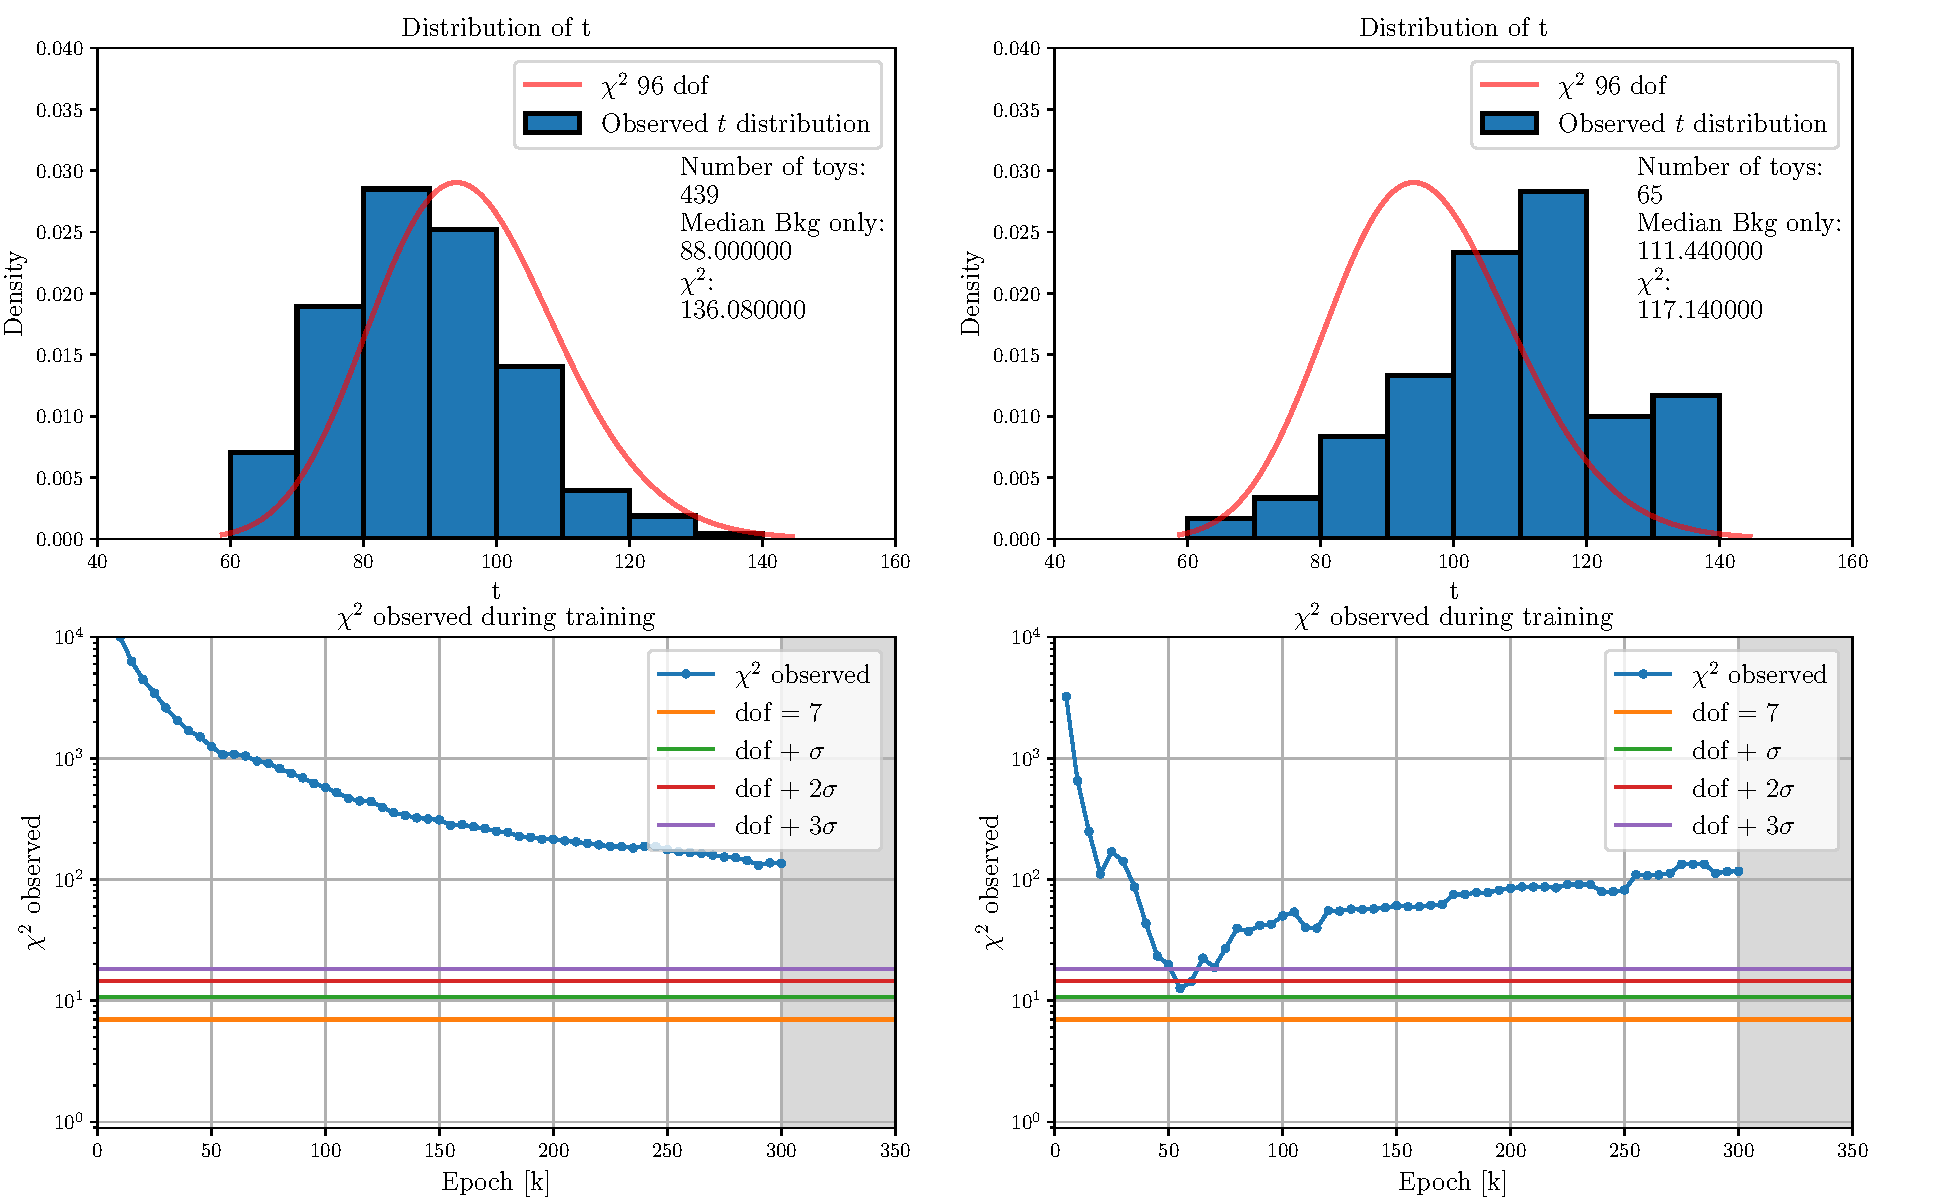
\includegraphics[width=1.0\textwidth]{Python/W_CLIP/wrong_wclip_2-2_3-0.pdf}
	\caption{Results for wrong choices of $W$ with \textbf{Zmumu-Zprime} dataset. On the left side there are the results for $N_\mathrm{ref}=200\si{k}$, $N_\mathrm{bkg}=20\si{k}$, $N_\mathrm{sig}=0$, $W=2.2$. On the right side there are the results for $N_\mathrm{ref}=1000\si{k}$, $N_\mathrm{bkg}=20\si{k}$, $N_\mathrm{sig}=0$, $W=3.0$.}
	\label{fig:WRONG_WCLIP}
\end{figure}